\renewcommand{\thechapter}{4}

\chapter{User Interactions and Permission Use on Android}

Our last chapter introduced interaction-based declassification
policies. However, it is unclear whether this matches user intuition
about how apps behave. In this chapter, I introduce a system for
studying how permission uses relate to user interaction within
apps. This system, named \apptracer{}, builds on the logging
facilities present in Redexer. It leverages logging and visualization
to help perform an app study over 150 top apps from the Google Play
store. I then follow this up with a 961-participant user study to
investigate how users understand permissions as they relate to the
UI. I found that the app's UI does deeply inform a user's expectation
that a permission will be used, but that the current implementation of
the Android permission system may mislead users under certain
circumstances.

\section{Introduction}

Android has a \emph{permission system} that asks users for
authorization before an app uses sensitive resources such as
contacts or GPS location.
% Older versions of Android asks users to approve a list of app
% permissions at install time, and Android~M improves on this with
% dialog boxes to request authorization at run time before the first
% use. However,
A key challenge in such authorization systems is balancing
user interruptions with making sensitive resource use transparent.
% Currently, Android uses either install-time lists of permissions or
% run-time dialog boxes to request authorization.
We hypothesize that Android's existing authorization systems
(install-time permission lists or run-time dialog boxes, depending
on the version) could achieve a better balance by integrating with the
app's user interface (UI), because the UI deeply informs the user's
mental model of the app's behavior, including security-relevant behavior.
%  If true, then Android's authorization
% system could use the UI to better balance user interruptions with
% making sensitive resource use transparent.

In particular, in this chapter we ask whether \emph{user
  interactions}---button clicks, page changes, dialog boxes,
etc.---can be taken as evidence of authorization to use certain
sensitive resources. If so, this could reduce the need for separate
authorization requests. Conversely, I ask whether sensitive resource
use without an associated interaction suggests a need for additional
authorization requests.
Note that while our studies are heavily influenced by Android, I believe the
results will generalize to related mobile OS's and
similar settings like web apps.

To answer these questions, I conducted two related studies. First, I
(and another grad studnet) reviewed 150 popular Android apps to
determine whether sensitive resource uses are related to user
interactions in existing apps.  If so, an authorization mechanism
integrated with the UI could work well with existing app designs.  To
carry out this study, we developed \apptracer{}, a dynamic analysis
tool that instruments Android apps to log UI actions and resource
uses, and then visualizes the logs as graphs that show temporal
ordering of logged events.
%\apptracer{} then visualizes such logs as graphs, where
%the nodes are UI actions or resource uses, and edges indicate temporal
%ordering. For example, a ``click'' node with an edge to a ``contacts''
%node indicates the users' contacts were accessed immediately after a
%click. 
We used \apptracer{} to determine whether each observed
resource use in each app was \emph{interactive}, meaning either it was
immediately preceded by a related UI event (e.g., accessing contacts
after clicking a button marked ``contacts''), or it was the main focus of
the current screen (e.g., using location on a map screen). 

We found that, across our subject apps, several resources (microphone,
camera, external storage, and calendar) are used almost exclusively
interactively; several others (including bluetooth and phone state)
are used mostly non-interactively (which we call in the
\emph{background} even if the app itself is on screen); and several
resources (most notably contacts and location) exhibit a mix of
interactive and background uses. These results suggest interactive and
background uses may call for different authorization mechanisms, and
that these mechanisms cannot necessarily be divided strictly by
resource.

% \jeff{loc is actually used interactively 40\% of the time, so I wonder
%   if it's really a good representative of that last category?}

These results informed the design of our second study, a
961-participant online survey investigating participants' expectations
about interactive and background permission uses. Each participant
viewed a slideshow of two usage scenarios for a mock mobile app, where
each scenario shows a short interaction (e.g., launching the app,
clicking a button, etc.) and then asks if the participant expects
microphone, location, and/or contacts to be used after the
interaction. We chose these resources to reflect a range of
interactivity as measured in our app study.  We aimed to gain insight
into how different factors
%(the resource and app being used and the type of interaction)
affect user expectations, and therefore which authorization mechanisms
might be appropriate for different usage patterns.
%
%In particular, we studied three hypotheses: whether users
%are likely to expect resources to be accessed after an interaction
%such as a button click; whether users expect background accesses of
%resources that are very common in apps; and whether users expect a
%resource to be accessed again if it was accessed before within an app.
%\jeff{Do we need prev?}

%In our study, we showed each participant a slideshow describing a
%typical usage scenario for one of two mocked mobile apps,
%\emph{HealthyFit Tracker} and \emph{FindMeCoffee}. Each scenario
%includes a pair of trials, where each trial shows a short interaction
%with the app (e.g., launching the app, clicking a button, etc) and
%then asks the participant whether they expect microphone, location,
%and contacts to be used after the interaction.

As we anticipated, we found that users are much more likely to expect 
resources to be accessed after a related interaction than in the 
background. However, we also found that seeing one 
interactive use does not prime the user to expect a future 
background use, indicating a potential weakness in the Android~M request-on-first-use 
authorization model. In contrast, our findings show that an 
authorization request at launch does increase expectations for 
both interactive and background accesses, perhaps because it better conveys the idea that 
the resource could be accessed at any time.

%an authorization request at launch does 
%increase expectations for later accesses. This has implications 
%for the Android~M permissions model's app
%users do not expect a background use if the previous use was an
%interactive use, but expectation does increase if authorization was
%requested when the app was launched.  Finally, we found users did not
%necessarily expect commonly used resources to be used in the
%background. \jeff{Do we want to give numbers for the above?}

Drawing on the results of our studies, we make three design 
recommendations. First, resource uses should be made after associated 
interactions as much as possible. Given the current makeup of apps, this 
should be achievable for many commonly used resources without extensive 
effort. Second, separate authorization dialogs might be unnecessary
for resources that are accessed mostly interactively (see, e.g.,~\cite{Roesner:2012}). 
Finally, authorization for background resource uses should be distinct 
from authorization for interactive uses, and these background authorizations 
may be most effective when the app is launched. 

%\kris{Mike said that we didn't point out that we were really defining
%  a new notion of context for these apps, more informed by the
%  implementation, and that that might lead us to be more plausibly
%  enforced via some security mechanism.}

% We found that users' expectation of resource use increased as they were
% shown more interactive access pattern.  Specifically, showing our participants
% a button click had the largest effect on their likeliness to expect a resource 
% use, more so than the impact of presenting an authorization request.  We 
% also observed that the relationship between real-world frequency and expectation
% was not consistent across all apps.  Our participants were likely to expect location 
% to be accessed frequently in the background and the microphone to be rarely 
% used outside of very interactive cases, which matched the results of our app 
% study. However, users did not expect their contacts to be accessed, which
% contradicts our previous findings.  Finally, we found that users are more likely 
% to expect a resource use in the background if they have previously seen an 
% indication of some background usage, such as a pop up notification indicating 
% that they are ``near a coffee shop'' which indicates the app accessed the user's
% location.  However, they were not more likely to expect a background use if 
% they were previously shown an interactive access even if an resource 
% authorization was presented on the first use.

% Based on the results of our studies, we observe that Android is
% already moving toward contextual security, and we recommend continuing
% in this direction. We found that many apps are already constructed so
% that, for very sensitive resources such as the microphone, access is
% already contextual in nature. Changing apps fit to this paradigm for most 
% resources would align apps with users' expectations.  Additionally, due to
% level of expectation we observed associated with highly contextual accesses, 
% authorization requests on interactive accesses would no longer be necessary.
% We also recommend more explicit authorization of background use as users 
% did not appear to be aware of all background resource accesses.

% meaning in a context with a clear UI action such as a button click. We
% also found that when resources are used in the background, it is
% typically to support foreground behavior, e.g., loading contacts
% asynchronously.  Finally, we found that location and phone identifiers
% (e.g., IMEI) are often used in the background and without notifying
% the user, typically to support advertising.  

% We also observed that apps only notified the user of a resource access
% when required to do so by Android M.  The vast majority of apps
% presented authorization requests directly before the first resource
% use and a few included a brief description for why they accessed the
% resource just before the standard Android M authorization dialog.  We
% used our observations to inform the construction of our user study.

% the log---was it after a button click, a page change, at app startup,
% in the background, or uncertain; and was there any authorization request,
% such as a modal dialog box with an alert message,
% prior to the use. %\jeff{What kinds of notifications were there?}

% Despite these changes, we observe that by not considering the user
% interface, Android's authorization approach
%  This paper aims to shed light on this hypothesis with two
% complementary studies. First, we ask the question, \emph{do existing
%   apps users permissions in an interactive manner?}, meaning, is it
% the case that there is typically a clear connection between user
% interactions with an app and access to sensitive resources. We
% partially answer this question by applying a dynamic analysis to 150 top apps
% from Google Play to determine 

% One advantage of the Android~M model is that it may allow users to
% better consider the
% \emph{context}~\cite{Nissenbaum:2004,Wijesekera:2015} before granting
% permission to an app.\footnote{There are also many other advantages to
%   the Android~M model, most notably allowing users to enable and
%   disable app permissions even after the app is installed.}  

% These are difficult questions to answer, and in this paper 
% In this paper, we conduct two complementary studies exploring how the
% context defined by user interactions---what window is on the screen,
% what buttons have been clicked, etc.---relate to actual and expected
% permission uses on Android. We measure actual permission uses in
% existing apps by analyzing the results of a dynamic program analysis.
% We measure expectations via a user survey.

% Mobile operating systems such as Android and iOS use permissions to
% protect access to sensitive resources including user data (e.g.,
% contacts) and device capabilities (e.g., GPS location). While
% permissions are conceptually simple, they suffer from a key
% limitation: once a permission to access a resource is granted, the app
% can access that resource for any purpose, at any time, unless and
% until the permission is manually revoked. Thus, apps that are
% legitimately granted permission for one purpose might misuse it for
% another.
%\jeff{add cites}.

% A potential remedy to this situation is to also consider the
% \emph{context}~\cite{Nissenbaum:2004,Wijesekera:2015} before allowing
% sensitive resource accesses. While contextual security has been
% considered before for mobile
% devices~\cite{Chen:13,Wijesekera:2015,Roesner:2012}, prior work uses
% shallow notions of context (e.g., is the app in the foreground or
% background) or focuses on how mobile operating systems or apps could
% be modified to better support context
% \cite{Roesner:2012,Roesner:2013,Ringer:2016}.

% Combining the results of these studies we identify a middle ground
% within the Android permissions landscape, wherein permission should be
% requested on each \emph{new} use of the permission. We call this
% pattern-based-access-control (PBAC). We found that pattern based
% access control could likely be used for almost all apps using
% microphone and video, and nearly all uses of contacts and external
% storage. For example, although a user may be fine with their contacts
% being accessed after clicking a button, they may not be comfortable
% with the same behavior happening each time the app runs. PBAC
% separates these two policies, and attempts to ask users about resource
% access in a minimally invasive way that still controls for their
% expectations.


% In this paper, we survey the context of resources uses in 150 top
% apps, and compare that to user expectations gathered in a
% medium-scale user study.  To perform our app study we developed
% \apptracer{}, a dynamic analysis tool that allows us to visualize app
% logs and understand where resources are used with respect to the app's
% UI. We used \apptracer{} to assign codes to each app corresponding to
% the set of resource access patterns we identified.

% Our user study attempts to understand whether the resource usage
% patterns apps use aligns with user expectations. We show users
% slideshows of app traces, testing various combinations of relevant
% events (such as pressing a ``find coffee'' button) and ask what
% resources they expect will be used. We test a variety of times (on app
% launch, after first use, never) at which users are presented with
% dialogs showing resources will be accessed. We test this for three
% resources (location, microphone, and contacts), and a variety of
% permutations of app scenarios.

% We set up our study to test the efficacy of the Android M (just in
% time) permissions model. It is well known \cite{Felt:2012soups} that
% install-time permissions are frequently ignored, but we posited that
% there may be some circumstances where no dialog was necessary because
% it was clear from context (e.g., contacts accessed after clicking on an ``add contact''
% button). We also posited that there may be circumstances under which a
% user is fine with authorizing some resource accesses, but then later
% wishes to revoke that access.

% Our app study identifies that some resources (such as microphone and camera)
% are almost exclusively used in an interactive way within top
% apps. Based on these results, we recommend that access use for these
% resources be tied to clearly identifiable UI elements, and other uses
% should be seen as suspicious. We identified another class of resources
% (contacts and external storage) which are frequently accessed in an
% interactive way, but for programmatic reasons may be accessed at a
% different time than a specific interaction. For example, an app may
% pre-fetch a list of contacts to be shown to the user later. Last, we
% found that some resources such as phone information (e.g., number and
% unique ID), location, and user accounts are frequently accessed
% without the user's knowledge. Based on the results of our user study,
% we found that these resources were less sensitive than others, but
% believe users should still be educated as to their collection.

% Combining the results of these studies we identify a middle ground
% within the Android permissions landscape, wherein permission should be
% requested on each \emph{new} use of the permission. We call this
% pattern-based-access-control (PBAC). We found that pattern based
% access control could likely be used for almost all apps using
% microphone and video, and nearly all uses of contacts and external
% storage. For example, although a user may be fine with their contacts
% being accessed after clicking a button, they may not be comfortable
% with the same behavior happening each time the app runs. PBAC
% separates these two policies, and attempts to ask users about resource
% access in a minimally invasive way that still controls for their
% expectations.

In earlier versions of Android, users were presented
with a list of permissions requested by an app at install time. The
user could then either grant the app full use of those permissions or
not install the app at all. This model had a number of
problems: few users comprehended or even read the list of permissions~\cite{Felt:2012soups},
and many apps requested more permissions than they used~\cite{Felt:2011}. 
Because of these
issues, Android M~\cite{AndroidMPermissions} switched to a model where
apps ask for a permission the first time it is needed; the permission is 
then granted indefinitely.
%%  This
%% brings Android closer to enforcing \emph{contextual
%%   integrity}~\cite{Nissenbaum:2004}, which states that resources
%% should be accessed in accordance with contextual norms.  
%However,
%on Android M, permissions are still granted indefinitely.

In our work, we ask whether authorization systems similar to
Android's can be improved by taking the user interface into account.
% In this paper, we study foundational questions about
% whether existing apps use permissions in a contextual manner
% (shedding light on whether asking for permission on the first use is
% necessary or sufficient); whether users expect permissions to be used
% contextually; and whether user expectations and current practice
% align. 
Note that our work is orthogonal to the question of whether
permissions are at the right level of granularity
\cite{jsjeon:spsm12,Bugiel:2013} or protect the right
resources~\cite{Felt:2012spsm}.

% Android security---particularly the permission system---has been
% heavily studied in the research community
% \cite{Felt:2011,Felt:2012spsm,Sarma:2012,Wang:2013,Chia:2012,Liu:2016,Balebako:2013,Fu:2014}
% (among many others). There is also substantial work
% \cite{Wijesekera:2015,Thompson:2013,Jung:2012} indicating that users'
% expectations about resource accesses depend on the context.

% Our paper builds on the prior work by studying the extent to which
% existing \cite{Ringer:2016,Micinski:2015,Yang:2013,Roesner:2012,Roesner:2013,Chen:13} contextual security systems could be applied to
% existing apps. Our paper also studies how app UI context influences
% user expectations about resource usage. We are unaware of other
% existing work that tries to answer these questions with similar
% studies. \jeff{Not sure how to word this.}

\paragraph*{Contextual Security on Mobile Devices}
%
% It has been repeatedly shown
% \cite{Thompson:2013,Jung:2012,Almuhimedi:2015,Balebako:2013,Fu:2014}
% that users are frequently surprised by resource accesses that happen
% while apps are in the background. For example,
%
The motivation for our work, that authorization can be better
integrated with the UI, exemplifies \emph{contextual
  security}~\cite{Nissenbaum:2004}, which suggests security decisions
should take the context into account. Several researchers have
studied contextual security on mobile devices. Almuhimedi
et. al~\cite{Almuhimedi:2015} showed users historical data about how
apps accessed their locations. They found 95\% of users reassessed the
apps' need for location, with 58\% of those users further restricting
location access.  King~\cite{King:2012} found users
are more likely to expect sensitive resource accesses when
suggested by the context. Felt et. 
al~\cite{Felt:2012hotsec} proposed a process for deciding the 
appropriate authorization mechanism for a permission based on the a
permissions' use in context. Several
researchers~\cite{Balebako:2013,Fu:2014,Wijesekera:2015} found users
are surprised by some sensitive resource accesses
%, such as location
%and phone information,
that occur when apps are in the
background. Most closely related to this paper, in a field study 
Wijesekera et al.~\cite{Wijesekera:2015} found that context is an
important factor in determining expectation of resource use.
Our work builds on this finding by using a controlled experiment 
to distinguish how different contextual factors, including consecutive 
interactions, contribute to user expectations.

The works just mentioned mainly define context as whether the
app is on or off the screen. In contrast, we use a
much richer notion of context based on sequences of UI actions. 

%While Wijesekera et. al~\cite{Wijesekera:2015} do perform
%a field study on a set of users and determine that context is an
%important factor in determining expectation of resource use, our work
%performs a controlled experiment across a variety of different
%variables. Specifically, our definition of app context is guided by a
%deeper notion of the sequence of actions a user took through an app
%(e.g., the sequence of clicks) whereas theirs only considers whether
%the app was on the screen at the time (and provides users a screenshot
%at that time to make decisions about if an access is expected). This
%also allows our study to reason about sequences of accesses and
%compare expectation about future access based on the expectation of
%the prior, incorporating aspects of the newer (Android M) architecture
%present in apps since that work took place.



% Wijesekera
% et. al~\cite{Wijesekera:2015} explored contextual integrity on Android
% and found that many users were surprised by some sensitive resource
% accesses that occur when Android apps are in the background. Flu
% et. al~\cite{Fu:2014} used run-time disclosures to show users which
% apps accessed their location. Many users were surprised to learn apps
% they did not frequently use accessed their location in the background.
% Balebako et. al~\cite{Balebako:2013} created the ``Privacy Leaks''
% tool, which allows users to audit which apps use their information in
% real time. They similarly found users were surprised that apps access
% location and phone information even when the apps had not been used
% much.



%  includes whether the app is in the background, but also recent
% actions in the app's UI.  Our paper complements the above studies by
% showing how an app's UI influences user expectations about resource
% usage.

\paragraph*{Enforcing Contextual Security}
Many systems have been proposed to enforce contextual security in
apps.  Chen et. al~\cite{Chen:13} present Pegasus, a static analysis
system for analyzing apps and enforcing policies based on
\emph{permission event graphs} (PEGs). For example, Pegasus can check
that contacts are only accessed after clicking a certain
button. PEGs inspired the design of \apptracer{}. However, \apptracer{}
uses dynamic (rather than static) analysis to reduce issues of false
positives---every behavior \apptracer{} logs occurred in an actual run,
whereas static analysis may report sensitive resource accesses that can never actually occur.
%conservatively overestimates the runtime
%behavior of the program (for example, it ).

% However, Permissions Event Graphs take into account a deeper knowledge
% of the Android API. \apptracer{}'s graph merely orders events
% temporally, with only a portion of edges coming from Android's
% semantics. This means \apptracer{} is less precise at understanding the
% program's behavior, but allows us to scale up to all of the Android
% API.

Yang et al.~\cite{Yang:2013} presented AppIntent, which uses symbolic
execution to determine sequences of UI events that lead to information
leakage. Micinski et. al~\cite{Micinski:2015} use symbolic execution
to enforce secure information-flow properties based on UI
events. While both systems are promising, in practice symbolic
execution is difficult to run at scale on Android apps due to the
complexity of modeling the Android framework.

Stiegler et al. developed CapDesk~\cite{capdesk} and later Polaris~\cite{Stiegler:2006}, 
two capability-based desktop system that utilize user interaction to drive access control.
However, CapDesk and Polaris's focus is limited to file access.
Roesner et. al~\cite{Roesner:2012} expand user-driven access control with \emph{Access Control
  Gadgets} (ACGs), which tie resource accesses to certain UI elements,
e.g., an ACG might allow location to be used only after a specific
button is clicked. ACGs were later expanded to work on Android, with 
and later without modifying the operating system~\cite{Roesner:2013,Ringer:2016}.
The original ACG paper includes a user study measuring 
expectations related to interactive permission uses; our work 
expands on this idea to study a broader variety of factors and 
use cases. 
%work on Android \cite{Roesner:2013} by modifying the Android runtime.
%Recent follow up work by Ringer et. al~\cite{Ringer:2016} allows ACGs
%to be used on an unmodified operating system. 
While the current paper
does not directly implement or measure ACGs, our findings do support
the use of ACGs.
% While our user study incorporates elements of the study
%done in the original paper on ACGs---specifically, we also measure
%expectation change as the result of clicks---we also measure user
%expectation across a larger possible design space encompassing
%different user actions and subsequent accesses.

\section{App Measurement Survey Methodology}

\begin{figure}[tb]
  \centering
  \includegraphics[width=.7\columnwidth]{leakfinder-chi2017/img/app-study-diagram.png}
  \caption{App Measurement Survey Procedure.}
  \label{fig:measurement-summary}
\end{figure}


In our first study, we reviewed a set of popular Android apps to determine
how UI actions and resource uses are related.
Figure~\ref{fig:measurement-summary} gives a high-level
overview of our review process, which ultimately produces
%  which uses \apptracer{}, a dynamic
% analysis and visualization tool we developed to show an app's UI
% events and permission uses.  Since
% \apptracer{}'s visualization is complex, two coders reviewed each
% visualization separately and then came to agreement for every app. The
%final result is
a set of \emph{resource use codes} that indicate, for each resource use,
what event (if any) caused the use. For example, we might
determine that in some app, contacts were accessed just after a button
click, or location was used immediately when the app launched.

The next subsections walk through the review process in detail.

% We wanted to understand and categorize the ways in which typical apps
% access users' resources. To do this, we surveyed 150 apps using a tool
% we built to help visualize the connection between UI interaction and
% use of sensitive resources. Using this tool, we applied an iterative
% manual-coding process to identify the set of resource-access patterns
% present in each app. Figure~\ref{fig:measurement-summary} shows a
% high-level overview of our process. In the following subsections, we
% provide details about the design and operation of our visualization
% tool, as well as our manual coding process.

\subsection{Binary Rewriting and Execution Logging}

The first step of our process uses \apptracer{}, a dynamic analysis tool
we developed. \apptracer{}
instruments the subject app so that, when run, it writes
a log of UI events and permission uses. \apptracer{} adds
instrumentation using Redexer~\cite{jsjeon:spsm12}, a
rewriting tool for Dalvik bytecode (the language
to which Android apps are compiled). Generally speaking, \apptracer{}
instruments code by appending a \code{log} method to the bytecode and
inserting calls to \code{log} at the beginning of UI-related callbacks
(e.g., \code{onClick} handlers for button events) and just before
calls to permission-protected methods (e.g., \code{getLastLocation}).

We identified methods associated with the UI using the Android
documentation. We identified permission-protected methods using the 
PScout dataset~\cite{Au:2012}, which attempts to list every
security-sensitive method and its associated permission. PScout also
includes information about sensitive content providers, intents, etc.
%
Note that while PScout is reasonably thorough, we found several cases
it missed. For example, we observed several visual
indicators of SD card use that had no corresponding log entry
\apptracer{}.  After
investigating the apps' decompiled code, we found the SD card was used
via Java IO methods omitted by PSCout. Whenever we found
such cases, we added the missing methods to our copy of the PScout
database and reran our evaluated apps.

% For example, we noted that PScout did not include methods in the
% popular Google Play Services API.

Once an app has been instrumented, a tester runs it to generate a log.
(Note that one log is usually sufficient because in most apps, any app
state is reachable from any other app state.)  We elide
the details of the log, but at a high level, for
each UI event, \apptracer{} records the type of event and the corresponding
parameters (e.g., what button was clicked, which menu option was
selected, etc.). For each permission use, \apptracer{} logs the name of
the called method and its arguments.

\subsection{Log Visualization}

\begin{figure}[tb]
  \centering
  \begin{subfigure}{.25\textwidth}
    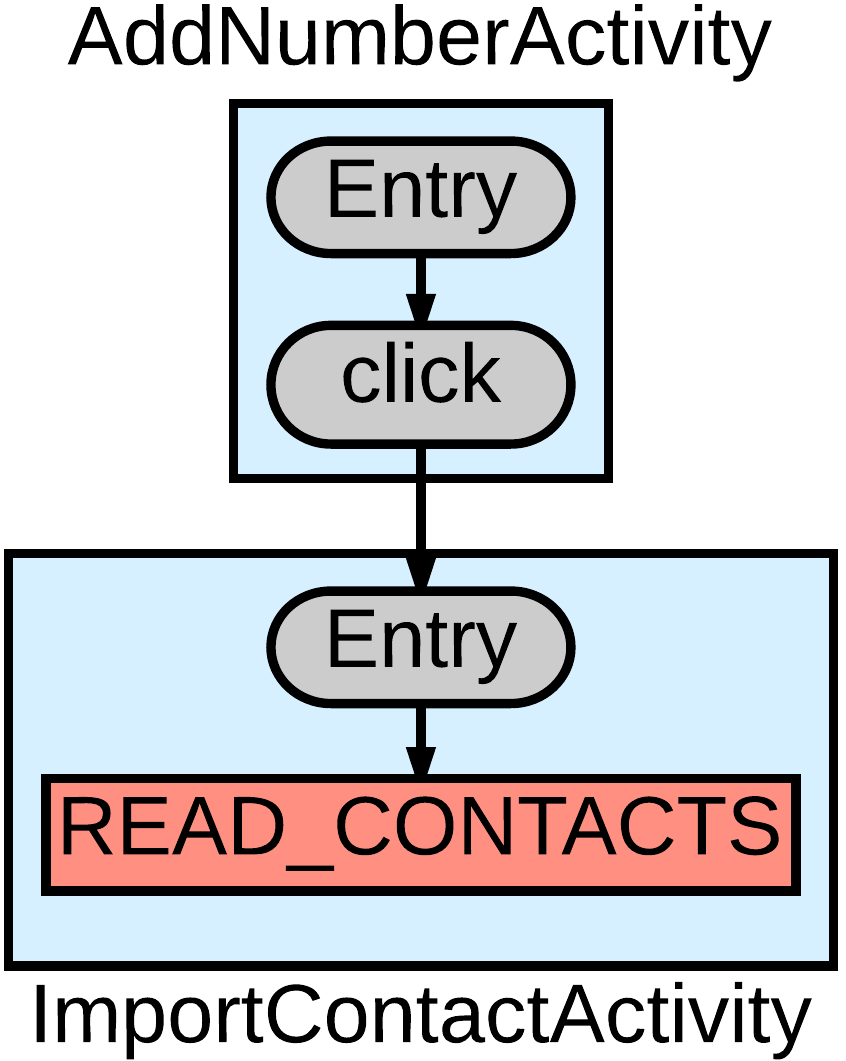
\includegraphics[width=\textwidth]{leakfinder-chi2017/img/click.png}
      \vspace{-.3in}
      \caption{Click}
      \label{fig:click}
  \end{subfigure}
  \begin{subfigure}{.25\textwidth}
    \vspace{-.1in}
    \includegraphics[width=\textwidth]{leakfinder-chi2017/img/uncertain.png}
    \vspace{-.3in}
    \caption{Uncertain}
    \label{fig:uncertain}
  \end{subfigure}

  \begin{subfigure}{.25\textwidth}
    \includegraphics[width=\textwidth]{leakfinder-chi2017/img/startup.png}
    \vspace{-.3in}
    \caption{Startup}
    \label{fig:startup}
  \end{subfigure}
  \begin{subfigure}{.25\textwidth}
    \vspace{-.1in}
    \includegraphics[width=\textwidth]{leakfinder-chi2017/img/bg-evt.png}
    \vspace{-.3in}
    \caption{Background-External}
    \label{fig:bg-ext}
  \end{subfigure}
  \caption{\apptracer{} graphs and corresponding resource access patterns in our codebook.}
  \label{fig:leakfinder-ex-graph}
\end{figure}

After the tester produces a log, the next step is log visualization.
Figures~\ref{fig:click}--\ref{fig:uncertain} show example
portions of \apptracer{}'s graph-based visualization, redrawn for
compactness and to omit most package names.
Here, light blue boxes represent
\emph{activities}, which are the ``screens'' of the
app. Within each activity, gray ovals represent the beginning
of that activity (``entry,'' which usually corresponds to the
\code{onStart} handler), UI events (e.g.,
``click''), or system events (e.g.,
\code{BATTERY\_CHANGED}).
Red rectangles indicate calls to methods
protected by the named permission. There is an edge from node A to node B if A
occurs immediately before B in the log. For example, in
Figure~\ref{fig:click}, contacts were read immediately after
the \code{ImportContactActivity} activity was started.

Since logs can be quite lengthy, \apptracer{} heuristically merges
nodes that arise from the same position in the bytecode. This
sometimes results in ambiguity. For example, in
Figure~\ref{fig:uncertain}, the single \code{onReceive} node actually
represents calls to an Android broadcast receiver that \apptracer{}
coalesced. We discuss this more below.

%  has been collapsed to
% represent multiple clicks within the activity.
% \kris{\apptracer{} *sometimes* disambiguates based on the resource
% identifier of the click, but not when a click handler is registered
% on multiple different objects, in that case you just check the
% receiver of the click, which we explain vaguely next}

Finally, \apptracer{} also allows the user to directly view the
log file entries corresponding to a node in the graph. This is
useful to retrieve more detailed information about the node. For
example, when reviewing Figure~\ref{fig:click}, we looked in the log
to determine that the clicked button had text associated with contacts.  As
another example, we used the logs to distinguish SD card accesses to
user files from accesses to the app's own storage. We do not count the 
latter as a sensitive resource access because it accesses data owned by 
the app. 
% This feature was 
% also used to determine whether or not reads/writes of the SD 
% card were made to files containing sensitive user information by 
% checking associated file path.  We only generated codes in situations 
% where user files were accessed to avoid over-counting when the app 
% simply saved its own information to the SD card.

\subsection{Resource Uses}

The next step is to examine the \apptracer{} graph and record a set of
codes that accurately categorize various resource accesses.
More precisely, for each red node in the graph, the coder
assigns a pair of the form $(\textit{resource}, \textit{pattern})$,
where \textit{resource} indicates what is protected by the permission
and \textit{pattern} is one of six different UI patterns, discussed
next.

To keep our results understandable, we grouped together resources
according to Google's permission
groups~\cite{permissiongroups}. For example, the single \code{SMS}
resource includes more fine-grained permissions such as \code{READ\_SMS} and
\code{SEND\_SMS}.
%\jeff{Are there additional permissions in SMS?}
%\dan{Yes, there's RECEIVE_SMS, RECEIVE_MMS, and a few others}

% This loss of precision conflates resource access but is
%consistent with current Android permissoin models.
% \apptracer{} does, however, provide us with insight towards each
% fine-grain resource within the permission groups which mitigates
% uncertainty that may arise while investigating apps.

We developed an initial codebook for UI patterns based on our
knowledge of Android app development. We then iteratively applied our
codebook to sets of five apps (not in our evaluation set) at a time
and adjusted the codes as necessary. After evaluating a total of
twenty apps, we felt we had reached a codebook with a minimal set of
orthogonal patterns.

% We arrived at this codebook based on our knowledge of Android app
% development and a preliminary analysis of a small set of apps. We used
% a content analysis based approach, starting with an initial set of
% codes we derived from the patterns we saw \apptracer{} generating and
% the concepts from related literature. We then iteratively applied our
% initial codebook to sets of five apps (not in our evaluation set) at a
% time, eventually evaluating twenty apps. We removed or regrouped
% redundant codes as appropriate, until we ended up with a codebook
% representing a minimal set of orthogonal patterns we saw in apps.

The six access patterns in our codebook are grouped into three categories.  First 
are the \emph{interactive} patterns \textit{Click} and
\textit{Page}. The code \textit{Click} indicates
resource use preceded by a UI event %interaction
 (including non-clicks such 
as swipes). For example, in Figure~\ref{fig:click}, we coded
\code{READ\_CONTACTS} as \textit{Click} because the contacts were
accessed on a straight-line path from the click of a button labeled as importing
contacts.
 \textit{Page} codes uses that are clearly associated with an activity
 but are not associated with exactly one
click.  For example, \emph{Page} would code the use of
  location during an activity that shows a
list of nearby stores.

Second, in the \emph{background} patterns \emph{Startup},
\emph{Bg-App}, and \emph{Bg-Ext}, the resource use has no obviously
connected user action. %interaction.
 \emph{Startup} codes a resource accessed
 right after app launch but before any screen appears
 (and is thus disjoint from \emph{Page}), e.g., the use of accounts in
Figure~\ref{fig:startup}, which occurs in a thread created at app
launch. \emph{Bg-App} codes a resource used while the app is
in the foreground, but with no clearly related user action.
%interaction.
 For example, a graph similar to Figure~\ref{fig:click} would be 
 coded as \emph{Bg-App} if a button labeled for importing contacts 
 was followed by the \code{GET\_ACCOUNTS} permission 
 rather than \code{READ\_CONTACTS}.
 \emph{Bg-Ext} denotes a
resource used due to a system event, meaning it would be used 
whether or not the app is on screen. For example, in Figure~\ref{fig:bg-ext},
accounts are read after the \code{BATTERY\_CHANGED} system event.

Finally, \emph{Uncertain} denotes a resource access that did not fit any
of the previous patterns. In Figure~\ref{fig:uncertain}, we see a
path from a system event to \code{onReceive} to \code{READ\_CONTACTS},
which should be coded as \emph{Bg-Ext}. But, the \code{onReceive} node also 
has an incoming edge from the click handler and the back button.
These uses would be coded as \emph{Bg-App}.
(The \emph{Click} and \emph{Page} codes do not apply 
because the associated buttons do not indicate contacts will be used.)
Because there are multiple possibilities, we code this case as \emph{Uncertain}.

If desired, an \apptracer{} user can subsequently review the logs to
try to resolve the 
uncertainty. For example, here the log entry associated with 
\code{BATTERY\_CHANGED} is followed by a call to
\code{onReceive} and then \code{READ\_CONTACTS}. Thus, the permission
use is coded as \emph{Bg-Ext}. We then separately looked at the log
entries for \code{click} and \code{back\_button}, and found they
were followed by an \code{onReceive} that was \emph{not} followed by
\code{READ\_CONTACTS}. Thus, examining the logs allowed us to
distinguish paths that we merged in \apptracer{}.

% Kris: This now sounds right to me. Maybe we should be more explicit
% about beating the reader over the head with this fact: just because
% there's an edge from BATTERY_CHANGED to onReceive, and there's an
% edge from onReceive to Click, and there's an edge from onClick to
% contacts, does *not* necessarily imply there is a transitive edge
% between them. Maybe this is worth pointing out more obviously?

Note that for each app we only count each $(\textit{resource},
\textit{pattern})$ pair once, no matter how often it occurs in the log.
A stronger notion of frequency would be hard to interpret, since it would
depend on how \apptracer{} heuristically coalesces graph nodes as well as 
to how the tester explored the app.
%, rather than indicating, e.g., the 
%frequency of accesses in a typical app execution.

% \subsection{Authorization}
 
% In addition to coding resource uses, we also used \apptracer{} to code
% the \emph{authorization level} for each resource used somewhere in the
% subject app. There are three possible authorization levels. \emph{On
%   First} codes that the app presented the user with a dialog asking
% for authorization at the first use of a resource (and not subsequent
% uses). \emph{On Launch} codes that the app asked for authorization
% once when the app was first launched. \emph{Never} codes that the app
% did not ask for authorization at run time (e.g., it was written for
% earlier versions of Android that asked for authorization at install
% time).

% \textit{Never} if the app did not notify the user of the resource
% access. This is possible in Android M either because the app was
% developed for an earlier API version or the resource is not part of
% one of Android's ``dangerous'' permission
% groups~\cite{dangerousperms}.  For example, if the app accessed the
% user's Bluetooth resource, Android M does not require and
% authorization dialog to be presented to the user.

% For example, if an app accessed location using a callback after the
% ``find coffee'' button was pressed, we assign it the code (Location,
% Click, Continuous). There are also limited cases where \apptracer{} does
% not give us enough information to decide the pattern being used. In
% these cases, we mark the pattern as undecided. We comment below when
% and why this happened and how we might improve \apptracer{}, but note
% that this happened relatively infrequently.

% For example, if an app's only access of location was after the ``find
% coffee'' button was pressed, and no notification was presented to the
% user, then we assign the tuple (Location, Never).

\subsection{Coding Apps and Resolving Differences}

Coding the resource uses of an app is inherently complex. Thus, two
coders reviewed apps independently in sets of 15 and met after
each set to resolve differences.  Coders took
approximately 10--20 minutes to code each app, and resolving
differences for a set of 15 apps took approximately 30 minutes.

Most differences between coders were due to one coder overlooking
a path or a resource in the \apptracer{} graph.
In almost all such cases, when the other coder pointed
out the omission, the first coder would quickly
reach the same conclusion as the other coder.
%
The remaining differences were caused by disagreements about whether
the resource use was interactive. For example, one app read a user's
accounts within an activity for filling a form. One coder
recorded this as \emph{Click}, since the accounts were read after a
click. The other coder recorded this as \emph{Bg-App}, because there
was no observable use of the account data, such as pre-filling the form with 
data from the user's existing accounts. After encountering several such
cases, the coders decided on a general principle of coding uses as
\emph{Bg-App} unless the UI explicitly mentioned that the resource
could be used---hence, this example was resolved as \emph{Bg-App}.

Inter-rater reliability between our coders for the non-visualization-error 
disagreements was Krippendorff's $\alpha=0.897$, indicating close agreement~\cite{kripalpha}.
% to measure the
%inter-rater reliability between our two coders for the non-visualization-error
%disagreements. We reached an $\alpha$ of 0.897, indicating close
%agreement.

%Jeff: I found the following mysterious. How would anyone know what
%the expected disagreement is? I suspect it's better to just say what
%conclusion to draw from the final alpha value rather than try to
%explain how the statistic works.
%using, which calculates the difference between the expected
%disagreement and observed disagreement between reviewers.
 
\subsection{App Selection}

We drew our subject apps from a larger set comprising the 20 top
downloaded free apps\footnote{as of June 11, 2016} from the
27 non-gaming categories on Google Play. We excluded gaming apps
because they typically use native code that \apptracer{} cannot
analyze. This yielded 503 apps (note there is overlap between
categories).

% We used top apps because we expect the behavior in
% those apps represents what users typically see.
% While it is likely that the patterns in these apps does not
% generalize to all apps, we expect that results about user
% expectations of permission usage will apply more generally.

We then randomly selected 150 apps to evaluate, subject to the 
constraint that no more than two apps were from the
same developer. (We wanted to avoid bias due to overrepresentation of
apps coded in the same style.). We excluded any 
apps that could not be run with \apptracer{}, replacing them with 
new randomly drawn apps to maintain an evaluation set of 150. 

We excluded 48 apps because Redexer fails when rewriting them and
\unusableerrors{} apps because either they refuse to run if modified
(due to internal or system signature checks) or they are primarily
implemented in native code. 
%Jeff: The Redexer/apktool difference is probably not important
% We excluded \redexererrors{} apps because Redexer fails
% when rewriting them and \apktoolerrors{} apps because they cannot be
% unpackaged and repackaged by the open source tool
% apktool~\cite{apktool}, which Redexer depends on. 
In most cases, we created accounts when signup was required to fully exercise an app, but we 
excluded \accountserrors{} apps because they require accounts that are hard
to set up online or require a fee (e.g., bank accounts).
%  performs checks that abort if its bytecode was
% rewritten; the app was preinstalled on our test devices \jeff{say what
%   model these are} and hence the modified version couldn't be
% installed due to a signature mismatch; or the app was primarily
% implemented in native code.



% Of the top Android apps, we found that a few developers, such as
% Google and the GO Dev Team, published a significant number of the top
% downloaded apps.  Therefore, We limit our maximum studied apps per
% developer to 2 to ensure that our results are not biased toward the
% set of best practices employed by a small number of companies.

%To get to 150 apps, we skipped \removedapps from our list of apps. We


\subsection{Limitations}

There are several potential limitations to this study. First, the tester
may miss some app behavior, leading to a log that omits
some possible resource uses and contexts. We tried to alleviate
this concern by exercising as much of the app as possible. However, we
did not use app features that required payment.

Second, \apptracer{} has limitations mentioned above: it may miss UI
events or permission-protected methods, and it merges nodes that
correspond to the same position in the bytecode. We tried to address
the former issue by looking for cases where we expected an event to be
in a log but it was not, and then adding the missing events or
methods. We addressed the latter issue by manually disambiguating some
of the uncertain cases.

% kris: We didn't really systematically do this, we just marked these
% cases as ``uncertain.'' Should we instead just say we marked them as
% uncertain, and since there were so few of them it was mostly fine?
% This is how we would resolve this problem if we were looking to use
% this tools to really dig into apps.

Third, our study reviewed only popular Android apps. Observing that a 
resource is already accessed interactively in 
popular apps would indicate that changing the Android framework 
or system to implement interactivity-related protections for those 
accesses may be reasonable. These apps also represent the 
common case and likely help to set user expectations about apps 
and permissions. However, we note that the apps we 
examine likely differ from the long tail of other apps in important ways; 
popular apps are likely implemented to high standards and unlikely to be 
malicious. We leave similar measurements 
on a broader set of apps as future work.

% Kris: better rewording here?

\section{App Measurement Survey Results}

\begin{figure}[t]
\centering % If we use something other than \columnwidth
\includegraphics[width=.6\columnwidth]{leakfinder-chi2017/img/Access_per_Resource_Groups.png}
\caption{Percent of observed patterns of each type, per resource. 
Bar labels indicate how many apps
  we observed using each pattern, non-normalized.}
\label{fig:access_per_resource}
\end{figure}

Figure~\ref{fig:access_per_resource} summarizes the resource use
patterns we found. For example, across all
apps, the camera was used in the \emph{Click} pattern 57 times. Orange-shaded 
bars indicate interactive use patterns, and 
blue shades represent background uses.  Resources are sorted 
by percent of interactive patterns.

We see that, to a rough approximation, the more sensitive the resource
the more likely it is used interactively. Indeed, microphone, media,
camera, and calendar were accessed almost exclusively
interactively. We investigated the background and \emph{Uncertain}
uses for these resources. One calendar use and the two SD card uses
were due to periodic background tasks (calendar syncing or scanning
for files). One camera use took a picture after the passcode was
entered incorrectly three times. One camera use and one calendar use
did not seem to access sensitive resources---the camera use accessed 
configuration information, and the calendar use got the current date
(which could be done without accessing the calendar). Finally, after
disassembling and reading the bytecode, we found one \emph{Uncertain} 
camera use could actually only happen interactively.

% Because these resources were accessed so infrequently in the
% background, we further investigated each app that exhibited this
% behavior by manually inspecting their bytecode.  The two background SD
% card uses were both periodic file accesses triggered by a user
% setting.  One app checked for malicious files and the other scanned
% for unused files to clear up storage space.  One app used the camera
% in the background to get the camera's configuration information and
% another took a picture of anyone trying to access the phone who
% incorrectly entered the passcode three times.  The third background
% case for camera was classified as \emph{Uncertain} due to limitations
% of \apptracer{}.  Because \apptracer{} coalesces like nodes, the graph
% included a path that indicated that the access could have been
% triggered by a background pattern.  However, on detailed manual
% analysis of the app we determined that this path cannot occur.  The
% first calendar background pattern was a periodic sync that occurred
% based on a user setting and the other access was the result of the app
% using the calendar to get the current date, unnecessarily requesting
% access to the user's resource instead of using a less sensitive
% method.

We next see that contacts, SMS, tasks, location,
and calls are used in a mix of interactive and non-interactive ways.
%(though note there are few uses of calls and SMS), making it
%hard to draw strong conclusions).
We investigated the background and
\emph{Uncertain} uses of these resources as well.
Contacts were used in the
background mainly to pre-fetch or sync the contact list. Two
apps used SMS in the background to listen for a registration
code after the user signed up for an account. Currently
running tasks were polled in the background to monitor
battery usage, scan for malicious apps, look for apps by the same
developer (to communicate with them), or for analytics and tracking purposes. 
Call-related permissions were
used in the background to block calls from a user-supplied blacklist.
While there were too many background location uses to examine them all,
those we did examine frequently 
had no obvious reason (as expected~\cite{Fu:2014,Almuhimedi:2015}), even in apps that elsewhere 
used location for a clear purpose.

% We also performed manual bytecode analysis to 
% investigate the background uses and found they were typically related 
% to the app's purpose, even when they did not inform the user resources 
% would be accessed. For example, the apps accessing calls in the background 
% did so to periodically access the call list and block calls the user previously 
% added to a blacklist. Contacts were mainly accessed in the background to
% pre-fetch or periodically sync the contact list.  We also observed two 
% keyboard applications that accessed contacts after the user began typing 
% although it did not appear that they actually used this data. Of the cases 
% marked \emph{Uncertain} for contacts and found that they arose due to the 
% same limitations discussed above.  In 4 cases, the correct accesses were 
% already marked by the coders and the other two cases should have been 
% marked background.  The two apps using SMS in the background
% did so to listen for a registration code after the user signed up for
% an account. The list of currently running tasks (i.e., apps), was polled
% in the background to monitor battery usage or scan for malicious apps,
% which we believe is legitimate because they could be disabled through
% user settings.  Apps also queried for running tasks to look for other apps
% by the same developer.  An example was a keyboard app that looked for
% add-on theme apps by the same developer which provided additional visual
% theme choices to the user if installed.  Other apps requested
% the list of running tasks in the background to use this information for 
% analytics and tracking purposes.  We again investigated \emph{Uncertain} codes 
% and found in all cases, \apptracer{} over-approximated the 
% number of resource accesses and all the correct accesses were 
% already marked by the coders.

Finally, four resources---accounts, power, bluetooth, and phone state
information---were mostly accessed in the background. We believe this
is either because developers believe users care less about these
accesses~\cite{Felt:2012spsm}, the uses are hard to explain
clearly to non-experts, or the uses are not naturally associated with
an immediately preceding interaction. 
% However, it may also be that--because of typical
%programming idioms--it is challenging to connect these uses to
%foreground interactions.

% Accounts similarly showed some clear uses, such as prefetching the
% user's email address, but also in many cases without a clear
% reason. Apps also frequently access power and bluetooth information in
% the background. Lastly, many apps access the user's phone information,
% likely for tracking users in contradiction to Google's recommendation
% to use an advertiser ID~\cite{GoogleAdId}.  We did attempt to refine
% the \emph{Uncertain} codes for these resource, but doing so could not
% significantly change our findings that these resources are more likely
% to be accessed in the background.

Looking in more detail at the breakdown between \emph{Click} and
\emph{Page}, we see that for most resources, \emph{Click} is a clear
majority of the interactive uses. The exception is location, which has
more \emph{Page} uses. This was mostly due to location use for
map screens or lists of nearby places. Breaking down
the background uses, we see the use of resources at \emph{Startup} and
in \emph{Bg-Ext} becomes much more common lower in the
chart.
%\jeff{Should we calculate some kind of correlation? More to say?}
%\kris{I think we agreed correlation is kind of silly due to small
%sample sizes and limited generalizability from the way we sampled and
%ran apps.}

% Looking at the interactive patterns across all resources, we see that
% \emph{Click} is much more frequent than \emph{Page}, which is sensible
% given their definitions. We looked at uses coded as \emph{Page} and
% found they generally occur when the activity is specifically dedicated
% to that resource, e.g., uses of the microphone to record the user
% speaking, or uses of location to display a map. Looking at the
% background patterns, \emph{Bg-App} is the most common. We believe this
% is because apps frequently perform access while on screen, whereas
% \emph{Bg-Ext} accesses happen less because the app is not performing
% UI-related processing. \jeff{That's not really an explanation, that's
%   just restating the observation in a different way...}\michelle{second 
%   jeff's comment here. also, can we compare this result to what serge 
%   found out re: background uses in some way?}

%\subsection{Authorization}

% \para{Authorization} 
% About half (49\%) of our subject apps were written for Android~M. We
% found that apps only requested permission to use a resource via the
% Android~M authorization mechanism. That is, no app written for pre-M
% Android requested runtime authorization, and no Android~M app
% requested authorization except with the Android~M mechanism. For
% example, no app gave reminders about resource use after the initial
% authorization or requested authorization to use \emph{non-dangerous}
% permissions.  (Android~M allows access to these without asking the
% user first).  We did find several cases where apps using Android~M
% would precede the Android~M dialog with a custom dialog explaining
% why the app was requesting authorization.  Finally, three Android~M
% apps requested authorization on launch even though the resources
% were not accessed until later in the app's execution.

\subsection{Resource Usage Across Apps}

\begin{table}
  \small
  \centering
  \begin{tabular}{c@{}c}
    \begin{tabular}{lr}
      \toprule
      \textbf{Resource} & \textbf{\# Apps} \\
      \midrule
      Location & 75 \\
      Media/SD Card & 69 \\
      Camera & 69 \\
      Phone State & 43 \\
      Accounts & 39 \\
      Bluetooth & 31 \\
      Contacts & 30 \\
      \bottomrule
    \end{tabular}
    &
    \begin{tabular}{lr}
    \toprule
      \textbf{Resource} & \textbf{\# Apps} \\
      \midrule
      Microphone & 14 \\
      Tasks & 13 \\
      Power/Diag. & 12 \\
      Calendar & 5 \\
      SMS & 4  \\
      Calls & 2 \\
       & \\
      \bottomrule
    \end{tabular}
  \end{tabular}
  \caption{Number of apps that used each resource.}
  \label{tab:per_app_resources}
\end{table}

We also measured the number of apps that used each resource at least
once, as a rough approximation for how familiar each resource is to
users.
% how commonly each resource is used, and 
%therefore with
Table~\ref{tab:per_app_resources} shows the results.
%shows the number of apps in our study used each resource. 
We found a 
wide range across resources, with little correlation between frequency of 
appearance in apps and usage patterns. For example, location was used 
frequently, and Figure~\ref{fig:access_per_resource} 
shows that it was often used in the background,
%Jeff: uncertain doesn't count as background.
whereas media/SD card was also used frequently, but was rarely 
seen in the background.
%   Conversely, the microphone was rarely used 
% (9\% of apps) and was never used the background, while the power/diagnostics 
% information was also rarely used (8\% of apps), but was often used in the 
% background (50\% of patterns).


\subsection{Discussion}

The results of our app survey suggest several
possibilities. Given the large amount of interactive resource use
overall, there seems to be a clear opportunity for better integrating
authorization into the UI. However, the question remains to what extent 
interactions make resource use apparent to users. We try to answer
this question in the next two sections.

Our app survey also shows that many resources are used in the
background, and many of these uses seem reasonable, at least to the
authors. Moreover, apps sometimes use the same resource both
in the foreground and in the background, to different purposes.
This suggests interactive and background uses should be authorized separately.
Thus,
in the next two sections, we also try to answer questions about how
background uses should be authorized, and about whether users'
expectations of interactive and non-interactive uses are related.

%Figure~\ref{fig:per_app_resources} gives the number of apps that use
%each resource at least once according to \apptracer{}.
%These counts are a rough approximation for how familiar users are with
%different resources. \jeff{Michelle, you probably have a better way of
%  saying the previous.}
%\jeff{The following discussion is not supported by the table, which
%  only lists the total \# of apps and does not split into
%  interactive/background. If we want to do the slit, I'd suggest three
%  columns, Int, Bg, Tot.}
%\jeff{Need to begin with some general point about the totals in the
%  table--overall, what does it show?}
%We found that resources could be divided into three categories based on the number 
%of apps we observed using them.  First, location, phone state, accounts, and bluetooth 
%were all frequently observed associated with background usage as described previously, 
%though the specific reason for use is unclear.  
%\jeff{The following two points don't really correspond with either the
%  table as-is or how we might change it to include interactive/background.}
%The camera, media/SD card, and contacts 
%are all used as part of functionality common to most apps, such as adding a 
%profile picture or sharing with friends.  Finally, the microphone, running tasks, 
%power/diagnostics, calendar, SMS, and calls were seen associated with functionality 
%specific to the app (e.g., calls was only used for call blocking apps).

%\michelle{in the user study we talk about overall frequency by resource,
%but we don't mention that here. should we? maybe the graph should indicate
%a total number of apps with uses on the right side of each bar so it's easy to compare
%frequent and infrequent resources? also distinguish \# of apps vs. \# of patterns?}
%\dan{I added the foreground and background totals to the right side of the graph, but
%it doesn't look great.  Does anyone have any ideas for a better way to present this
%or do we think this helps?}
%\kris{I thought we wanted to talk about the number of apps exhibiting these things too, which isn't really helped by this chart}

% Additionally, we found that no app notified the user of accesses to
% resources outside the set of Android's ``dangerous'' resource groups.
% 49\% of our studied apps conformed to the Android M permission model
% and requested authorization to access ``dangerous'' resources prior to
% the first use and the remaining apps provided no notifications.  Of
% the apps that provided an authorization dialog, three apps requested
% authorization on launch even though the resources were not accessed
% until later in the app's execution.  Finally, we observed that there
% were no cases where the app notified the user of a resource access
% after the first use.

\section{User Expectations Study Methodology}

\begin{figure}[t]
\centering \includegraphics[width=.5\columnwidth]{leakfinder-chi2017/img/fig4vertical.png}
\caption{User expectations study procedure. Lower 
portion shows partial examples of user actions and survey questions.}
\label{fig:survey-example}
\end{figure}

After our app survey, we conducted an online study to elicit
users' expectations about resource use as different user actions are
performed on a smartphone.
%interactions.
 Our goal was to understand to what extent user
expectations align with the interactivity patterns we
observed in our app study. Concretely, our user study examined the following three
hypotheses:

\emph{H1. Users are more likely to expect resource accesses with an
  interactive use pattern than without.}

\emph{H2. The more apps that use a resource (as measured in our app survey), the more 
likely users are to expect less-interactive uses of that resource.}

\emph{H3. Users are more likely to expect resource accesses they
  have seen before.}

Note that \textit{H1} and \textit{H3} have implications for the Android~M
permission system. Specifically, if \emph{H1} is true, users already
expect a resource to be accessed due to user action, so an
explicit authorization request may be unnecessary. Additionally, if
\emph{H3} is false, then users granting authorization for a resource
in one access pattern does not cause them to expect that resource to
be used later in a different pattern. Thus, requesting authorization
only on first use may be insufficient.

\textit{H2} is a proxy for a more general hypothesis: that 
users are more likely to expect accesses to resources with which they
are familiar. Familiarity is likely affected by many factors including
how many apps use the resource and how often they do so, whether
passive notifications are present (as for location), coverage in the
news media, etc. For simplicity, we use the frequencies in
Table~\ref{tab:per_app_resources} as a metric of familiarity.

\subsection{Study Overview}

We recruited participants through Amazon's Mechanical Turk
crowdsourcing service. All participants were at least 18 years old and
located in the United States. Participants were paid \$1.00 for
completing the survey. The survey was approved by the University 
of Maryland IRB. Participants were instructed that we
wanted their opinions about an app; privacy and sensitive resources
were not explicitly mentioned.

Figure~\ref{fig:survey-example} gives a flowchart of the procedure
followed by each study participant. First, the participant reads a
short description of an app.  We used two mock
apps in our study: FindMeCoffee (\coffee{}) and HealthyFit Tracker
(\fitness{}).  FindMeCoffee locates nearby coffee shops, allows
users to share the location of favorite coffee shops with friends, and
supports ordering coffee via voice command. HealthyFit Tracker tracks
workouts, allows sharing workouts with friends, and allows posting
audio ``smack talk'' on the user's profile. Note while these apps
demonstrate different categories, we do not attempt to fully study
the effect of app type on user perceptions.

Next the participant views one sequence of user interactions with the
app, shown as a
slideshow of app screenshots. To avoid confusion with terminology in
the next section, we refer to such a sequence as a \emph{user action}.
 For example, in the user action in
Figure~\ref{fig:survey-example}A, the user clicks the bottom-most
button (outlined in red), and the app then displays an authorization
request dialog. In Figure~\ref{fig:survey-example}C, which is only
shown partially, the user exits the app and returns to the device home
screen.

After viewing a user action,
%interaction,
the participant answers
five-point Likert questions such as those in Figure~\ref{fig:survey-example}B, which
ask whether a resource is ``Definitely not'' to ``Definitely
yes'' accessed immediately after the user action.
To avoid priming the user, the survey asks about 
camera,
SMS, flashlight, ``accessing
credit card information,'' and ``looking up coffee shop reviews'' (\coffee) 
or ``reading your heart rate'' (\fitness) as well as the 
three resources we study.
%The survey asks about three resources we study:
%microphone, location, and
%contacts. To avoid priming the user, the survey also asks about
%camera,
%SMS, flashlight, ``accessing
%credit card information,'' and ``looking up coffee shop reviews'' (\coffee) 
%or ``reading your heart rate'' (\fitness).

% The participant was next shown one resource access event, defined by
% the resource being used and its access pattern. She then answered
% questions about the current behavior of the app, such as whether the
% app is currently ``accessing your location" or ``listening through
% your microphone," with answers on a five-point Likert scale from
% ``definitely not" to ``definitely yes." These questions included the
% three resources we were primarily interested in (detailed below), as
% well as three additional resources and two auxiliary actions (such as
% ``accessing credit card information"), all included as controls.

Next, the participant answers five distractor questions, views another user action,
 and answers the same Likert questions about the second
user action. The distractors are designed to induce a cognitive break
and ensure the two access patterns are treated as separate events. 
For example, one distractor asks users ``Which button would you press if 
you wanted to find a new coffee shop?''
We did not measure the effectiveness of distractors.
The
participant concludes the survey by answering demographic questions.
Participants took 4 minutes and 45 seconds on average to complete the survey.

% Two example slideshows and associated surveys are included in the
% supplemental materials. 
% \jeff{Are there supplemental materials with the final version? If not, cut.}
% \michelle{I believe yes? We should get info about this.}
%\jeff{Make sure we submit this!}
%\kris{Rock is very on top of this.}

To understand the effect of resource access patterns on user
expectation, we analyze responses about the first user action each
participant viewed. We use responses about the second user action to
examine how prior exposure affects expectation.


%\michelle{not sure if i have successfully standardized terminology here}

\subsection{Conditions}

%\jeff{Sometimes we separate things with -, sometimes with : (next
%  section), and sometimes we just juxtapose things. We should be
%  consistent. Normalizing this section to -.}

Participants were assigned round-robin to one of 42 conditions, which varied across four variables: 
the \textit{app}, the \textit{resource} being accessed, the \emph{authorization pattern}, and the pair of \emph{interaction (int) patterns}.\footnote{Through this section we will use the abbreviation int.\ pattern to avoid 
confusion with the interactions in our regression analysis.}
Table~\ref{tab:scenario} lists possible values for 
each variable, and conditions comprise one value from each column. 
%We label 
%each condition using the abbreviations for its application, resource, authorization pattern, first 
%access pattern, and second access pattern, respectively. 
\begin{table}[b]
{
\singlespacing
\centering 
\begin{threeparttable}
\begin{tabular}{c c c c}
    \textbf{App} & \textbf{Resource}\tnote{1} & \textbf{Authorization}\tnote{2} & \textbf{Int.\ Patterns}\tnote{3} \\
    \toprule
  \coffee & \mic & \first & \colorbox{yellow}{\interactive-\interactive}\tnote{4} \\
  \fitness & \colorbox{yellow}{\contacts}\tnote{4} & \launch & \interactive-\backgroundonly \\
   & \location & \never & \backgroundnotify-\backgroundonly \\
   & & & \colorbox{cyan}{\backgroundonly-\backgroundonly}\tnote{4,5} \\
    % 				       & \multirow{2}{*}{\mic} & \multirow{2}{*}{\first} & \colorbox{yellow}{\interactive - \interactive} \\
    % \coffee & \multirow{2}{*}{\colorbox{yellow}{\contacts}} & \multirow{2}{*}{\launch} & \interactive - \backgroundonly \\
    % \fitness & \multirow{2}{*}{\location} & \multirow{2}{*}{\never} & \backgroundnotify - \backgroundonly \\
    %     				& & & \colorbox{cyan}{\backgroundonly - \backgroundonly} \\
    \bottomrule
\end{tabular}
   \begin{tablenotes}
     \small
      \item[1] \mic{} - Microphone, \contacts{} - Contacts, \location{} - Location
      \item[2] \first{} - First, \launch{} - Launch, \never{} - Never
      \item[3] \interactive{} - Click, \backgroundnotify{} - Background w/Notif., \backgroundonly{} - Background Only
      \item[4] Only used with \coffee
      \item[5] Only used with \launch
   \end{tablenotes}
\end{threeparttable}
\caption{Possible values for each variable in tested conditions.}
\label{tab:scenario}
}
\end{table}

As mentioned earlier, our study used two mock apps, FindMeCoffee and
HealthyFitTracker, and three resources, chosen to cover a range of int.
 patterns observed in our app survey: Microphone (\mic, 
only interactive accesses observed), Contacts (\contacts, mixed interactive and 
background uses observed), and Location
(\location, also mixed).

Our study considered three different authorization patterns. 
First use (\first) mimics Android~M, presenting an
authorization dialog during the first user action but not the
second. Launch (\launch) presents an authorization dialog immediately
after the app's home page is shown, but before any further screenshots.
We noticed anecdotally that a few apps in our study used this strategy.
Never
(\never) does not show any authorization dialog at run time. This
mimics older versions of Android.

% Finally, we considered three authorization patterns that reflect
% implementation in current apps; this allows us to examine how
% authorization affects user expectations on initial and subsequent
% resource accesses. First use (\textit{\first{}}) presents an
% authorization dialog to the participant after the first access
% pattern, but before our expectation questions. This pattern models the
% intended ``ask-on-first-use" operation of Android M.  Launch
% (\textit{\launch{}}) presents an authorization dialog to the
% participant directly after the app's home page is shown, but before
% any access patterns are presented. This models our observation that
% some apps request all permissions immediately, even if they do not use
% a given resource until much later.  Never (\textit{\never{}}) presents
% no authorization dialogs to the participant at any point. This models
% apps built for older versions of the Android API, which for
% compatibility reasons do not request resource authorization during
% runtime.

We examined three different int.
 patterns, also
drawn from the app survey: Button Click (\textit{\interactive{}}),
Background with Notification (\backgroundnotify, uses a resource without 
interaction, but displays an icon and short message in the notification 
drawer indicating some condition is met, such as being located near a coffee shop)
and Background Only 
(\backgroundonly, uses a resource in a way not clearly shown in the UI). 
We can order these from most (\interactive) to least
(\backgroundonly) interactive. We always label the
button clearly for its use (no deception). We
do not test UI widgets besides buttons.

% is most interactive. We note that for the study, the button is clearly
% labeled for its associated action; we do not test cases where the
% button is deceptive. Background with Notification
% (\textit{\backgroundnotify{}}) displays a continuous but passive
% visual cue (e.g., an icon in the system tray) indicating the access is
% occurring.  \michelle{add figure if room}. In Background Only
% (\textit{\backgroundonly{}}), which is least interactive, the resource
% access is not related to the user interface.


%We did not observe any resources only used in the background. \michelle{is that true? what about like 
%IMEI? do you mean to say we didn't include all-background resources in the user study?}\dan{There were 
%no resources seen who had 0 foreground uses.  IMEI, could be a case for that, but we didn't look at the resources 
%at that granularity, so it would fall into READ\_PHONE\_STATE, which was used multiple times in the foreground 
%to auto fill account signup forms with the user's phone number.}

% For example, if location is accessed 
%when the user navigates to a screen without any visual cues related to location, it is in this category.
%\michelle{put multi resource background only here vs. below? revisit.} We define the interactivity ordering of our accesses patterns as \textit{\interactive} > \textit{\backgroundnotify} > \textit{\backgroundonly} because \textit{\interactive} requires direct user interaction, \textit{\backgroundnotify} provides a visual cue to the user, but not direct interactivity, and \textit{\backgroundonly} provides no indication to the user of access.

Regardless of a participant's assigned condition, the survey always
asks about expectations for all resources and auxiliary actions.
As a result, we implicitly collect data about users' expectations for the
\backgroundonly{}-\backgroundonly{} int. pattern pair, with authorization pattern \never{}, for the two non-targeted 
resources in each condition. For example, a participant assigned to the \coffee{}-\mic{}-\first{}-\interactive{}-\interactive{} 
condition also answers Likert questions about contacts and location that are analyzed within the 
\coffee{}-\contacts{}-\never{}-\backgroundonly{}-\backgroundonly{} and \coffee-\location{}-\never{}-\backgroundonly{}-\backgroundonly{} 
conditions. 
%We ask for the users' expectations regarding access of all three tested resources no matter
%  the resource in question for the specific scenario.  Therefore, we also collect data about the users' 
%  expectations regarding the scenario with the same app, authorization pattern \textit{\never}, and pair of access
%  patterns \textit{\backgroundonly}, \textit{\backgroundonly} for the resources not explicitly tested by the scenario.

Testing the full-factorial combination of all variables was
infeasible, so we eliminated conditions that were redundant or less
relevant to our hypotheses, resulting in 42 final
conditions.
%
In more detail:
We exclude conditions where the second int. pattern is more interactive than
the first, as we assume 
the participant's second expectation would be dominated by the second int. pattern, rather than by the  
combination of patterns.
We use \backgroundnotify{} only in the first user action, because we
  are primarily interested in its effect on user 
expectations for the second user action. We assume expectations for \backgroundnotify{} itself will 
depend entirely on whether the participant notices the passive cue, a topic that has been well studied~\cite{Sunshine:2009tn,Schechter:2007bj}
but is somewhat orthogonal to our work. These two rules limit the int. pattern pairs we study to those
in the last column of Table~\ref{tab:scenario}. 

We exclude \never{}-\backgroundonly{}-\backgroundonly{} conditions because they provide no 
evidence of resource use, and are therefore identical to the implicit scenarios discussed above. 
We also exclude \first{}-\backgroundonly{}-\backgroundonly{} because, in our experimental 
design, they are indistinguishable from \launch{}-\backgroundonly{}-\backgroundonly{}. In Table~\ref{tab:scenario}, 
\backgroundonly{}-\backgroundonly{} is highlighted in blue to indicate that it is only used with the 
\launch{} authorization pattern. 

Because we do not comprehensively consider the effect of app type, we limit \fitness{} conditions to those
we anticipated would have the largest variation in expectations. Specifically, we consider only \location{} and \mic{} 
and only conditions where the two user actions exhibit different int. patterns. The \fitness{} scenarios therefore 
include all combinations of variables in Table~\ref{tab:scenario} that
not are not highlighted in blue or yellow.
%
%We developed an online study where participants were shown one of 42 unique sets of interactions 
%with a mock smartphone app.  Each slideshow involves one particular resource utilization and exhibits 
%two interaction patterns.  Additionally, in some instances a pop-up notification is shown requesting 
%access to a particular resource.  Figure~\ref{fig:survey-example} gives an example slideshow where
%the user sees the the Microphone resource used interactively and is asked to authorize the app's use
%directly before the access.
%
%After each interaction pattern, we ask participants to answer 8 questions about their expectations 
%regarding what the app was doing. Six actions focus on common resource usages we observed during our 
%app survey such as is the app ``accessing your location'' or ``listening through your microphone.'' Two 
%auxiliary actions are not related to resources such as ``accessing credit card information'' and ``looking 
%up coffee shop reviews.'' Each action expectation is based on a five-point Likert scale ranging from 
%``definitely not'' to ``definitely yes''.

%After capturing the participants' expectations from the first interaction pattern, we include a set of distractor questions to induce cognitive breaks before asking for participants' expectations regarding a second interaction pattern.
%
%These breaks are a means to separate in a participant's mind any ongoing effects of the first access pattern from the second.  For example, the participant could expect that clicking a button uses the phone's GPS location to find a nearby coffee shop and is still using the location when you leave that screen because it takes some time to pull the GPS coordinates, but not because the second access pattern actually caused another location access. Finally, we conclude the survey with a set of demographics questions.  

%\subsection{Recruitment}


\subsection{Statistical Analysis}

To test \emph{H1} and \emph{H2}, we primarily consider the expectations expressed by participants
after the first user action. We use a logistic regression, appropriate for ordinal Likert data, to 
estimate the effect of the app, resource, authorization pattern, and
int. pattern on participants' expectation. 
%
To test \emph{H3}, which concerns the effect of the prior user action, we also use a logistic regression,
with participants' expectation for the second user action as the outcome variable. We use the same input 
factors as before, this time including both int. patterns.

Each regression includes multiple observations of each participant: the explicit condition plus two implicit 
\never{}-\backgroundonly{}-\backgroundonly{} responses. As is standard, we include
a mixed-model random effect that groups observations from the same participant~\cite{hedeker2008}.

Our initial model for each regression included the input variables plus all possible two-way interaction terms. To 
prevent overfitting, we tested all possible combinations of these inputs and selected the model with 
minimum Akaike Information Criterion (AIC), a standard measure of model quality~\cite{akaike1974}. 
We present only the final model for each regression.  

\subsection{Ecological Validity and Limitations}

We use a controlled experiment with mock apps. While this limits ecological validity, it allows 
us to reason statistically about the effect of specific factors on participants' expectations, and to 
disregard factors such as participants' history with an app or reputation of the app's developer. 
In a study environment, participants may be less suspicious 
than if their real data were at risk. To partially account for this, we ask about expectation rather 
than comfort level~\cite{Rao:2016}. 

By limiting our survey to two apps and restricting the int. patterns
and resources tested, we likely miss factors, and particularly combinations 
of factors, that influence expectations. As one example, users likely expect 
SMS and Calls to have different usage patterns, and these expectations may 
vary with app type.
However, based on the results of our app survey, 
we believe the variables chosen still provide useful insights.

Each participant sees two user actions in a relatively short 
time period. We do not
study the effect of longer sequences of actions or
long-term use (e.g., over days or weeks) of an app.

As is typical for online studies and self-reported data, some participants may not take the survey 
seriously, and some may try to complete the survey multiple times. We limit repeat participants 
using MTurk ID and browser cookies. While MTurk has generally been validated for high-quality 
data~\cite{Buhrmester2011,Kittur2008,Downs2010,Toomim2011}, U.S. MTurkers are
somewhat younger and more male, tech-savvy, and privacy-sensitive than the general population, 
which may limit the generalizability of our results~\cite{Kang2014}.

These limitations apply similarly across all conditions; we therefore consider comparisons among conditions 
to be valid. 
 

\section{User Expectations Study Results}

We now present the results of our online user study.  We found that
\emph{H1} holds: users were the most likely to expect a resource use
when shown a more interactive int. pattern. In contrast, we observed 
that while resource type does affect user expectation, \emph{H2} 
was not strongly supported. 
%We found little evidence 
%for \emph{H2}, but we did observe that resource type does affect 
%user expectation. 
Finally, we found that \emph{H3} does not hold. However, our results 
indicate that both background notification (\backgroundnotify{}) and 
on-launch authorization requests (\launch{}) increase user expectation 
of future resource accesses. 
%users are more likely to expect 
%that users were more likely
%to expect a resource use after the second user action whenever they
%previously saw a background notification (\backgroundnotify{}) or
%on-launch authorization request (\launch{}).

For each of our hypotheses, we present
key findings from our regression analysis.  Summaries of our regressions are shown in 
Tables~\ref{tab:regression1} and~\ref{tab:regression2}. Each table shows the included 
input variables and their values. Each variable includes a \emph{base
  case} value (identified by dashes in the remaining columns).
The odds 
ratio (OR) shows the observed effect of each value relative to the base case, measured as odds 
of expectation increasing one unit on our Likert scale. We also provide the 95\% confidence 
interval (CI) and $p$-value for each measurement. 

For example, the third row of Table~\ref{tab:regression1} shows that switching from \backgroundonly{}
to \interactive{} in the first user action, all other variables held constant, is associated 
with a 106.3$\times$ likelihood of increasing one unit of expectation. The CI expresses 95\% confidence 
that the ``true'' odds ratio is between 63.6 and 177.7. A $p$-value less than 0.05 is interpreted as 
statistically significant. 

The second 
half of each table shows interactions between value pairs, given as the two values 
separated by a colon. These odds ratio indicate the 
change in likelihood when the two variables co-occur, relative to considering them independently. For 
example, the \location{}:\interactive{} odds ratio of 0.2 in Table~\ref{tab:regression1} suggests the combined effect of 
these two values is \emph{subadditive}: only 20\% 
as strong as predicted by their individual effects.

\subsection{Demographics}
A total of 961 participants completed the study. Participants' ages ranged from 18 to 70+ years, with  
37\% age 18-29. Fifty-three percent reported being male and 47\% female. (``Prefer not to answer''
and ``other'' options for gender were provided.) Participants were required to be from the United States. Forty-five 
percent of participants reported holding a college degree, and 25\%
reported having ``far above average'' smartphone expertise.
Each condition had at least 20 unique participants. Twenty people dropped out partway through the survey, 
distributed evenly across conditions. 


%20 participants did not complete the survey.  Our dropouts were evenly distributed across scenarios.
%
% Incomplete data from survey
% 23 participants did not complete
% Of which, 3 were rejected re-attempts
% 1 completed the entire survey but failed to submit
% nearly all the rest quit after the app description slide
% 10 coffee app, 13 fitness app
%

\begin{table}[t]
\centering
\begin{threeparttable}
\small
\begin{tabular}{l l r c r}
    \textbf{Variable} & \textbf{Value} & \textbf{Odds Ratio} & \textbf{CI} & \textbf{$\boldsymbol{p}$-value} \\
    \toprule \toprule
     App & \coffee & -- & -- & -- \\
            & \fitness & 1.3 & [0.96, 1.78] & 0.086\\
     \midrule
     \multirow{3}{*}{Int} & \backgroundonly{} & -- & -- & -- \\ 
     					      & \textbf{\interactive{}} & \textbf{106.3} & \textbf{[63.6, 177.7]} & \textbf{< 0.001*} \\
                    				     & \textbf{\backgroundnotify{}} & \textbf{4.1} & \textbf{[2.6, 6.7]} & \textbf{< 0.001*} \\
     \midrule
     \multirow{3}{*}{Res} & \mic{} & -- & -- & -- \\
     				    & \textbf{\location{}} &  \textbf{17.5} & \textbf{[13.4, 22.9]} & \textbf{< 0.001*} \\
                          		    & \contacts{} & 0.8 & [0.6, 1.0] & 0.056 \\
     \midrule
     \multirow{3}{*}{Auth} & \never{} & -- & -- & -- \\
     				     & \textbf{\first{}} & \textbf{2.2} & \textbf{[1.2, 4.0]} & \textbf{0.008*} \\
					          & \textbf{\launch{}} & \textbf{1.9} & \textbf{[1.2, 3.2]} & \textbf{0.008*} \\
     \midrule \midrule
     \multirow{3}{*}{App:Res} & \coffee{}:\mic{} & -- & -- & -- \\
     					   & \textbf{\fitness{}:\location{}} & \textbf{0.4} & \textbf{[0.3, 0.6]} & \textbf{< 0.001*}\\
					   & \fitness{}:\contacts{} & 1.1 & [0.8, 1.7] & 0.546\\
     
     \midrule
     \multirow{5}{*}{Res:Auth} & \mic{}:\never{} & -- & -- & -- \\
     						& \textbf{\contacts{}:\launch{}} & \textbf{3.2} & \textbf{[1.5, 6.7]} & \textbf{0.002*} \\
     							         & \contacts{}:\first{} & 1.5 & [0.6, 3.6] & 0.41 \\
							         & \location{}:\launch{} & 0.8 & [0.4, 1.6] & 0.487 \\
							         & \location{}:\first{} & 0.5 & [0.2, 1.3] & 0.166\\
    \midrule
    \multirow{4}{*}{Res:Int} & \mic{}:\backgroundonly{} & -- & -- & -- \\ 
    							& \textbf{\location{}:\backgroundnotify{}} & \textbf{2.4} & \textbf{[1.2, 5.0]} & \textbf{0.021*} \\
    						        & \textbf{\contacts{}:\backgroundnotify{}} & \textbf{5.0} & \textbf{[2.3, 11.3]} & \textbf{< 0.001*} \\
						        & \textbf{\location{}:\interactive{}} & \textbf{0.2} & \textbf{[0.1, 0.4]} & \textbf{< 0.001*} \\
						        & \textbf{\contacts{}:\interactive{}} & \textbf{0.2} & \textbf{[0.1, 0.4]} & \textbf{< 0.001*} \\
    \bottomrule \bottomrule
\end{tabular}
\begin{tablenotes}
     \small
     \item \textbf{*}Significant effect 
      \hspace*{2cm}
      \textbf{--} Base case (OR=1, definitionally)
   \end{tablenotes}
\end{threeparttable}
\caption{Summary of regression over participant expectations after the first
  user action.}
\label{tab:regression1}
\end{table}

\begin{table}[t]
\small
\centering
\begin{threeparttable}
\small
\begin{tabular}{l l r c r}
    \textbf{Variable} & \textbf{Value} & \textbf{Odds Ratio} & \textbf{CI} & \textbf{$\boldsymbol{p}$-value} \\
    \toprule \toprule
     \multirow{2}{*}{Int 2} & \backgroundonly{} & -- & -- & -- \\     
     						& \textbf{\interactive{}} & \textbf{810.4} & \textbf{[352.2, 1864.9]} & \textbf{< 0.001*} \\
     \midrule
      \multirow{3}{*}{Int 1} & \backgroundonly{} & -- & -- & -- \\
      					    & \interactive{} & 1.0 & [0.8, 1.4] & 0.9\\
					    & \textbf{\backgroundnotify{}} & \textbf{2.1} & \textbf{[1.5, 2.8]} & \textbf{< 0.001*}\\
     \midrule
     \multirow{3}{*}{Res} & \mic{} & -- & -- & -- \\
     					& \textbf{\location{}} & \textbf{20.0} & \textbf{[15.5, 25.9]} & \textbf{< 0.001*} \\
     					    & \contacts{} &  1.0 & [0.8, 1.3] & 0.768 \\
     \midrule
     \multirow{3}{*}{Auth} & \never{} & -- & -- & -- \\
     					& \first{} & 1.4 & [0.9, 2.4] & 0.174 \\
					          & \textbf{\launch{}} & \textbf{1.7} & \textbf{[1.1, 2.7]} & \textbf{0.027*} \\
     \midrule \midrule
     \multirow{5}{*}{Res:Auth} & \mic{}:\never{} & -- & -- & -- \\
     						 & \textbf{\contacts{}:\launch{}} & \textbf{4.4} & \textbf{[2.2,8.5]} & \textbf{< 0.001*}\\
     						   & \contacts{}:\first{} & 2.1 & [1, 4.5] & 0.056\\
						   & \location{}:\launch{} & 0.8 & [0.4, 1.5] & 0.445\\
						   & \textbf{\location{}:\first{}} & \textbf{0.5} & \textbf{[0.2, 0.9]} & \textbf{0.029*}\\
     \midrule
     \multirow{3}{*}{Res:Int 2} & \mic{}:\backgroundonly{} & -- & -- & -- \\							
     							& \textbf{\location{}:\interactive{}} & \textbf{0.1} & \textbf{[0.03, 0.3]} & \textbf{< 0.001*}\\	
     							   & \textbf{\contacts{}:\interactive{}} & \textbf{0.03} & \textbf{[0.01, 0.1]} & \textbf{< 0.001*}\\
     \bottomrule \bottomrule
\end{tabular}
\begin{tablenotes}
     \small
     \item \textbf{*}Significant effect 
      \hspace*{2cm}
      \textbf{--} Base case (OR=1, definitionally)
   \end{tablenotes}
\end{threeparttable}
\caption{Summary of regression over participant expectations after the second
  user action.}
\label{tab:regression2}
\end{table}

\subsection{H1 -- Interactivity v. Expectation}
We found that \textit{H1} holds: the more interactive the int. pattern, the more likely the 
user is to expect the resource access. In fact, interactivity (specifically \interactive{})
is the strongest indicator of expectation we measured.

Table~\ref{tab:regression1} shows that both \interactive{} and \backgroundnotify{}
significantly increase the likelihood the user expects a resource access compared to \backgroundonly{}.
The effect of \interactive{} is particularly strong (OR 106.3, $p< 0.001$). Because the confidence intervals of \interactive{} and \backgroundnotify{} do not overlap, we can also conclude \interactive{} generates
significantly more expectation than \backgroundnotify{}.  Table~\ref{tab:regression2} confirms that the strong 
association between \interactive{} and expectation holds for the second user action as well (OR 810.4, $p < 0.001$).
%
\begin{figure}[b]
  \centering
  \includegraphics[width=.7\columnwidth]{leakfinder-chi2017/img/LikertCharts.png}
\caption{Likert-scale expectation responses for (a) the first user action, organized by 
int. pattern, and (b) the second user action, organized by authorization pattern.}
\label{fig:vars_vs_expectation}
\end{figure}
%
Figure~\ref{fig:vars_vs_expectation}a illustrates this finding, showing that 90\% of 
participants who saw a \interactive{} int. pattern first definitely or probably expected 
the associated resource use, compared to 72\% for \backgroundnotify{} and 25\% 
for \backgroundonly{}.
%In more detail, figure~\ref{fig:vars_vs_expectation}(a) shows the percentage 
%of responses given for each Likert scale option for each interaction pattern type.  
%Shades of green indicate a ``Yes'', shades of red indicate ``No'' and the grey indicates 
%``Unsure'' responses.  90\% of survey takers who saw a \interactive{} interaction pattern 
%responded ``Def Yes'' or ``Prob Yes'', whereas only 72\% indicated the same for \backgroundnotify{} 
%and 25\% for \backgroundonly{}.

Explicit authorization, which is by definition interactive, is also associated with a significant increase in expectation.
Compared to \never{}, both \first{} and \launch{} have odds ratio effects of about 2$\times$ 
for the first user action (Table~\ref{tab:regression1}), both significant. This result makes intuitive sense, as the dialogs for both 
(\first{} and \launch{}) occur very closely in time to the first int. pattern. 


%shows the percentage of each response on our Likert scale with 
%each colored bar associated with an access type from the first set of accesses.  For example, Figure~\ref{fig:access_vs_expectation} shows that ~75\% of all participants who were shown a button click responded ``Definitely Yes'' when asked if the resource for their scenario was accessed.  
%Figure~\ref{fig:access_vs_expectation} further shows that expectation increased as the interactivity of the access pattern increased.

%We also observe \textit{\interactive{}} is the strongest indicator of user expectation.  No other variable's confidence interval overlaps with \textit{\interactive{}}'s.  For the first access, \textit{\location{}}'s ceiling is 41.8, whereas \textit{\interactive{}}'s floor is 43.3.  Similarly, for the second access, \textit{\backgroundonly{}} for the previous access 
%has a ceiling of 2.8, whereas \textit{\interactive{}}'s floor is 352.2, showing that \textit{\interactive{}} has a larger impact than any other variable.

\subsection{H2 -- Real-World Frequency v. Expectation}

We observed an inconsistent relationship between real-world frequency and
expectation. Location was the most frequently seen 
resource in the app study (75 apps according to Table~\ref{tab:per_app_resources}) and was also the most expected 
resource we tested. As shown in Tables~\ref{tab:regression1} and \ref{tab:regression2}, \location{} was
associated with 17-22$\times$ higher likelihood of expectation compared to \contacts{} (seen in 30 apps) or \mic{} (seen in 14 apps).
%JF: Changed from %'s to absolute numbers because the #'s are in the tables.
%($16.1\times$ and $17.5\times$, respectively, for the first user action; OR 20.0 each in the second user action). 
Non-overlapping CIs and $p$-values less than 0.05 indicate these
effects are significant. This is consistent with \emph{H2}; however,
as our frequency measurement is only a very rough approximation
of user familiarity, we note that this effect could relate to existing passive
notifications for location, the higher volume of academic and
media coverage of the location permission, or other factors.

However, \emph{H2} does not hold when comparing \contacts{} and \mic{}. While 
\textit{\contacts{}} was seen about twice as often in the app study, there was no 
significant difference in expectation between the two resources, at either the first or second user action. 
This could be because our app frequency metric does not sufficiently capture differences (or in this case, 
similarities) in users' overall exposure to each resource.

While there was no significant difference between the main effects of \contacts{} and \mic{}, 
we found evidence that users rarely expected \mic{} to be used with 
\backgroundonly{}. Looking at the \textit{Res:Int} interaction in Table~\ref{tab:regression1}, 
\location{}:\backgroundnotify{} and \contacts{}:\backgroundnotify{} both show significant 
superadditive results, indicating that these combinations are even more expected, relative to 
the baseline \mic{}:\backgroundonly{} combination, than those factors' main effects would predict. 
We hypothesize this difference is driven more by low expectation for background microphone 
access than high expectations for the other combinations. 
The interactions involving \interactive{} are significantly 
subadditive, but we suspect this is a ceiling effect: expectations for \interactive{}, 
which as shown in Figure~\ref{fig:vars_vs_expectation}a are very high, cannot increase beyond the end of our Likert scale. We see similar effects for the \interactive{} interactions in Table~\ref{tab:regression2}.  

%This observation is 
%consistent with \emph{H2} as it suggests \mic{}, which was uncommon in our app study (14 apps in Table~\ref{tab:per_app_resources}), is not expected to be used with \backgroundonly{} interactions.

%effects when seen together (3.9 odds ratio, 0.02 p value and 3.1 odds ratio, < 0.04 p value respectively).  
%\textit{\location{}:\interactive{}} and \textit{\contacts{}:\interactive{}} both had significantly sub-additive effects when seen
%together (0.3 odds ratio, 0.01 p value and 0.1 odds ratio, < 0.01 p value respectively) and 
%\textit{\location{}:\backgroundnotify{}} and \textit{\contacts{}:\backgroundnotify{}} both had significantly super-additive 
%effects when seen together (3.9 odds ratio, 0.02 p value and 3.1 odds ratio, < 0.04 p value respectively).  We saw 
%a similar relationship in Table~\ref{tab:regression2} for the interaction \textit{Res:Access 2}, where 
%\textit{\location{}:\interactive{}} and \textit{\contacts{}:\interactive{}} both had significantly sub-additive effects when seen together (0.1 odds ratio, < 0.01 p value and 0.03 odds ratio, < 0.01 p value respectively).
%Because \textit{\mic{}:\backgroundonly{}} is more unexpected than the main effects independently would suggest, 
%we expect that this caused the interactions including \textit{\backgroundnotify{}} to appear more expected and the interactions with \textit{\interactive{}} can not move any higher up the Likert scale, so it looks like they are not as expected when compared to \textit{\mic{}:\backgroundonly{}}.

\subsection{H3 -- Effect of Previously Seen Accesses}

To examine the effects of prior accesses on participants' expectations, we focus on Table~\ref{tab:regression2}. 
Overall, we find that \textit{H3} does not hold: participants are not
  more likely to expect resource accesses they 
have seen before. In particular, the int. pattern variable \textit{Int1:Int2} does not appear in the final 
model, suggesting the combination of int. patterns does not meaningfully influence expectation at the 
second user action.

However, participants did appear more likely to expect a background access if they had previously 
seen an indication that background accesses might be used. Table~\ref{tab:regression2} shows expectation at the second user action was significantly higher when the first int. pattern was \backgroundnotify{} (OR 2.1, $p<0.001$) or 
the \launch{} authorization request was shown (OR 1.7, $p=0.027$), both of which indicate that 
background access may occur. Figure~\ref{fig:vars_vs_expectation}b
illustrates this finding, showing that in the second user 
action, more participants definitely or probably expected resource usage in \launch{} conditions (47\%)
than in \first{} (42\%) or \never{} (22\%). 
Additionally, the superadditive relationship between \launch{}
and \contacts{} in both regressions may suggest a \launch{} request primes users to 
expect non-interactive accesses to contacts. 

In contrast, we found evidence that the authorization pattern \first{}
implies only a single access.  Table~\ref{tab:regression2} shows that
\first{} did not have a significant effect ($p = 0.174$) compared to
\never{}, indicating that an authorization associated with the first
user action is no more effective than no authorization when thinking
about a second user action. The subadditive relationship between
\location{} and \first{} (OR 0.5, $p=0.029$) also suggests that
authorization requests associated with a specific event train users to
only expect a resource access after an authorization request. This
decreases the otherwise relatively high expectation of background
location access. These relationships, while not particularly strong,
are notable because they imply that the Android~M model may in some
cases be counterproductive; we explore this further in the Discussion
section below.


\subsection{App v. Expectation}
Finally, we observed that the app type did have some effect on the way other variables were perceived. 
We found no significant difference between the two mock apps with respect to the first user action ($p=0.086$), 
and app effects did not appear in the final model for the second user action, suggesting no meaningful 
relationship with expectation. However, we do observe in Table~\ref{tab:regression1} a significant, subadditive relationship 
between \textit{\fitness{}} and \textit{\location{}}, indicating that location accesses were less expected in the fitness app 
than the coffee app. We expect that across a wider variety of apps, further relationships between app type and expected resource usage would be observable. 

%
% p value) and the variable was removed from the model completely when considering the 
%second access because it had no disernable effect.  However, the interaction between \textit{\fitness{}} and \textit{\location{}} had a sub-additive effect (0.2 odds ratio, < 0.01 p value).  The relationship between 
%\textit{\fitness{}} and \textit{\location{}} indicates that the app does effect users' expectations, though due 
%to the limited number of apps tested we are unable to test the full extent of the relationship between 
%app and expectation.

\section{Conclusions and Design Recommendations}

Based on our app survey and user study, we propose several ways
to improve Android's and similar authorization systems.

\subsection{Access Resources As Interactively As Possible}

Our app study found that camera, microphone, media, and calendar are
already used almost exclusively interactively
in popular apps. Moreover, our user study
found that users overwhelmingly expect resource access after an
explicit click on a related item. We speculate that users would also
have higher expectations of resource access under other interactive uses.
% To keep our user study tractable it
% does not cover other interactive uses, but we speculate that users would also
% have higher expectations of resource access under such uses as well.
%app study's broader definition of interactivity.

Thus, we recommend expecting (or perhaps even requiring) most or all
accesses to these four resources to be interactive.  Other
resources are more frequently used in the background, and it is not
always obvious how to associate their uses with a foreground
interaction. However, we argue that developers should prioritize (and
the Android framework should encourage) making background uses
more interactive when possible.  For example, a social media app that periodically 
pulls the user's contacts to recommend new friends could tie this background
access to a foreground interaction by asking the user to ``turn on'' this feature 
at launch and provide a settings menu where the user could turn the feature off
at a later time. 
%\michelle{and perhaps a periodic reminder that it is turned on? 
%not for every access, but maybe every couple of months?}
While this design is similar to the authorization mechanism 
provided by Android M, implementing it in the app provides context, which 
we have found is important to decision making.

We also recommend that when resources that are more typically used interactively 
will be used in the background, these uses should be
documented explicitly in the app's description or a similar
user-visible location.
%\michelle{, to set users' expectations appropriately}.

% \michelle{does this fit here? not sure}
% While we did not explicitly test users' reactions to the \emph{Page} pattern, 
% we hypothesize that it would have similar effects on expectation, and that 
% it could be encouraged and enforced using similar mechanisms.

\subsection{Use Interactions to Grant Authorization}

Our results further suggest that if a resource use is interactive, then a separate
authorization dialog can be eliminated.  We speculate that removing
explicit authorization requests in these cases could reduce potential user 
confusion (e.g., ``I just clicked `Import Contacts,' why is it asking 
me if I want the app to access contacts?''). In addition, removing 
these requests could reduce annoyance and habituation, 
potentially helping the user to focus on other, less clear 
authorization decisions. Eliminating request dialogs for interactive 
use cases could also help motivate developers to prioritize 
interactivity, as mentioned above.  
Of course, to handle potentially malicious apps we must be sure the
preceding interaction is clearly related to the resource use.
%Any enforcement mechanism must also deal with the concern that the app
%UI cannot deceive users.
For example, clicking on a location icon
should not cause the camera to be used. 
% ACGs offer one solution to
% this problem by offering a limited set of UI elements tied to
% permissions that developers integrate into their apps.
%JF: We said all of that above, why repeat here?

We envision two main approaches to enforce this principle. One
idea is access-control gadgets~\cite{Roesner:2012,Roesner:2013}, which
we discussed with Related Work. 
% Is it appropriate to instead use ACGs here, since it has already
% been defined above? Is it redundant to cite those papers again?
Another approach would be to leave
apps as they are, but use a program analysis to ensure they
conform. For example, we could use \apptracer{} to do so, in one of two
possible modes. \apptracer{} could be run ahead of time, e.g., by an app 
market gatekeeper, to examine app behavior. Even though it would not necessarily observe all app behavior,
results from analyzing behaviors users actually encounter would still
be useful. \apptracer{} could also be used for auditing: power users and 
security experts could use
\apptracer{} to log an app's behavior as they use
it and then retroactively check the \apptracer{} graphs for any
suspicious behavior, which could then be reported to the broader public.

\subsection{Handle background authorization separately}

We found that users were much less likely to expect background
resource access if authorization dialogs were presented after a prior
user action or were not presented at all. Thus, we recommend requesting
authorization separately and explicitly for background uses. Based on
our study, it may be preferable to do so when apps are first
launched. However, because our study showed the increase in expectation is
small (especially compared to the expectation after a click), it
may be important to also show background notifications of use (which
also increased expectation) so users remain aware.
We note that while authorization on launch informs many 
users that background accesses should be anticipated, 
Figure~\ref{fig:vars_vs_expectation} suggests there are others who 
do not recognize this possibility. 
Further research into the best approach is still needed.

Resources that have a broad mix of interactive and background
uses---such as contacts---might particularly benefit from separate
background authorization and limited requests for interactive
uses. This could help avoid potential misconceptions about interactive
uses being the only uses.

% For resources such as contacts, for which both interactive and background 
% uses are common, clearly distinguishing authorization for background access 
% (in combination with limited requests for interactive access as described above) 
% could help avoid misconceptions about interactive uses being the only uses. 

Future work could shed light on how differences in background use cases 
affect user expectations and preferences. For example, users might be expected 
to react differently when contacts are accessed in the background for pre-fetch 
(a use case identified in our app survey) compared to advertising. We also
expect that the frequency of access will impact the user's
  decision. For example, it may be possible to tie high-frequency background uses to some 
foreground passive notification (e.g., a notification tray icon), similarly to the design presented 
by Balebako et al. for informing the user of data leakage~\cite{Balebako:2013}. This could 
make the user aware of the accesses without requiring additional authorization effort.
%\michelle{also uncommon / more scary background could be authorized explicitly when it happens 
%with minimal effort, vs. high-frequency which will need a more streamlined solution}
% In cases
%where access occurs frequently in the foreground, interactivity could lower the
%burden on the user to authorize those uses. More work is needed to understand h%ow
%frequent background uses should be handled. We suspect that
Program analysis tools such as \apptracer{} could potentially be used to 
separate these cases and apply different authorization policies accordingly.

We thank the anonymous reviewers,  This research was
supported in part by NSF CNS-1064997, a UMIACS contract under the
partnership between the University of Maryland and DoD, and a Google
Research Award.
